% main.tex — Compound Bias in LLM-as-a-Judge: A 2×2 Factorial Study
% Target venue: EMNLP 2025  |  Template: ACL LaTeX
%
% Compile:
%   pdflatex main.tex
%   bibtex main
%   pdflatex main.tex && pdflatex main.tex
%
% Figures are loaded from ../figures/  (relative to this file).
% Tables are hard-coded from results/tables/*.csv values.

\documentclass[11pt]{article}
\usepackage[hyperref]{acl2023}   % swap for acl2025 when released

% ── Core packages ─────────────────────────────────────────────────────────────
\usepackage[utf8]{inputenc}
\usepackage[T1]{fontenc}
\usepackage{graphicx}
\usepackage{amsmath,amssymb}
\usepackage{booktabs}            % \toprule \midrule \bottomrule
\usepackage{multirow}
\usepackage{xcolor}
\usepackage{hyperref}
\usepackage{natbib}
\usepackage{microtype}
\usepackage{array}
\usepackage{caption}
\usepackage{subcaption}

% ── Figure path ───────────────────────────────────────────────────────────────
\graphicspath{{../figures/}}

% ── Convenience macros ────────────────────────────────────────────────────────
\newcommand{\eg}{\textit{e.g.}\xspace}
\newcommand{\ie}{\textit{i.e.}\xspace}
\newcommand{\etal}{\textit{et al.}\xspace}
\newcommand{\pval}[1]{$p{=}#1$}
\newcommand{\fstat}[2]{$F{=}#1,\;p{=}#2$}
\newcommand{\etasq}[1]{$\eta^2{=}#1$}

% ─────────────────────────────────────────────────────────────────────────────
\title{When Two Biases Compound:\\
       Position and Verbosity Bias in LLM-as-a-Judge Evaluation}

\author{
  Haroon Maqbool \\
  \texttt{haroon@example.com}
}

\begin{document}
\maketitle

% ═══════════════════════════════════════════════════════════════════════════════
\begin{abstract}
TODO (write last, after Results are finalised).
LLM-as-a-Judge systems are widely used for scalable evaluation, yet
their susceptibility to compound biases---interactions between
positional preference and verbosity preference---remains unstudied.
We present a 2$\times$2 factorial experiment across 5 judge models,
3 datasets (MT-Bench, SummEval, Urdu MT-Bench), and
% TODO: update N after re-running consolidate.py with deduplication fix
% (original 5,753 included duplicate rows from re-runs of experiment.py)
\textbf{[N]}~evaluation
decisions. All five judges exhibit \textit{super-additive} compound
bias ($F{=}\textbf{[F]},\;p{<}10^{\textbf{[exp]}},\;\eta^2{=}\textbf{[eta]}$), meaning the
simultaneous presence of both biases inflates decision errors
beyond the sum of individual effects. We release all code and data.
\end{abstract}

% ═══════════════════════════════════════════════════════════════════════════════
\section{Introduction}
\label{sec:intro}

TODO. Motivate the study. Cite \citet{zheng2023judging} for MT-Bench,
\citet{wang2023faireval} for position bias, \citet{raina2024judgebench}
for judge reliability. State the gap: no prior work studies how multiple
biases \emph{interact}. Summarise contributions (2--3 bullets).

% ═══════════════════════════════════════════════════════════════════════════════
\section{Related Work}
\label{sec:related}

TODO. Cover: (1) LLM-as-a-Judge \citep{zheng2023judging},
(2) position bias \citep{wang2023faireval},
(3) verbosity/length bias, (4) JudgeBench, RobustJudge.

% ═══════════════════════════════════════════════════════════════════════════════
\section{Experimental Design}
\label{sec:design}

\subsection{2$\times$2 Factorial Structure}

We cross two binary factors:
\textbf{Position} (which response appears first in the prompt: \textsc{First}/\textsc{Second})
and \textbf{Length} (which response is longer: \textsc{Short}/\textsc{Long}).
This yields four conditions per question--judge pair.
Figure~\ref{fig:design} illustrates the design.

\begin{figure}[h]
  \centering
  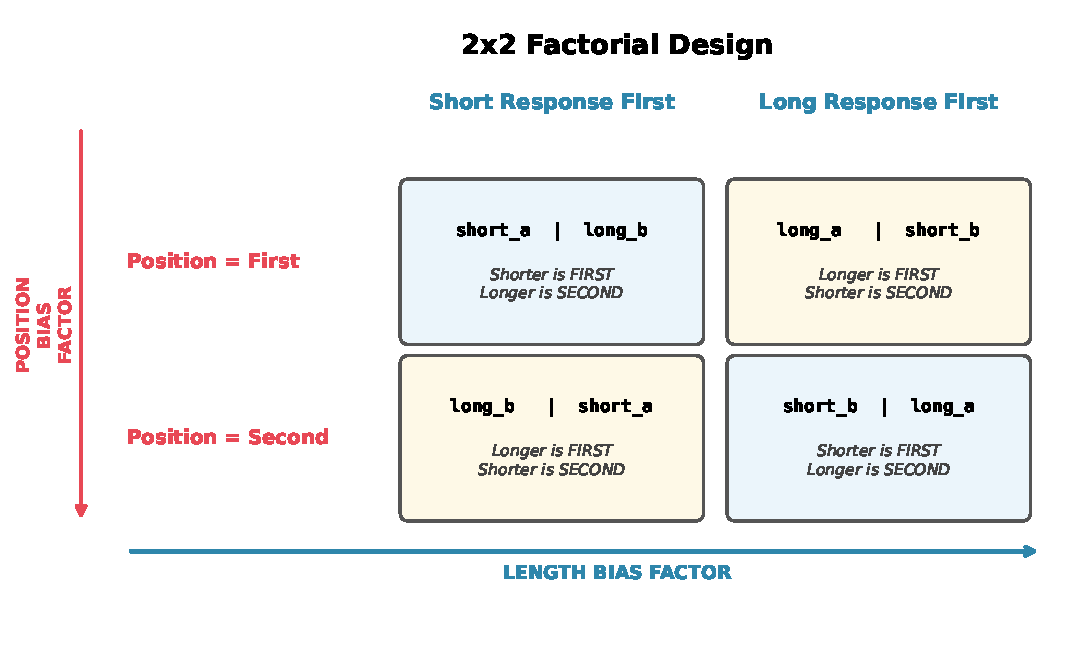
\includegraphics[width=\linewidth]{fig1_design_diagram.pdf}
  \caption{The 2$\times$2 factorial design. Each cell shows which
           variant occupies the Response~A and Response~B positions
           in the judge prompt. \texttt{short\_a}/\texttt{long\_a}
           are short/long rewrites of the original response~A;
           \texttt{short\_b}/\texttt{long\_b} for response~B.}
  \label{fig:design}
\end{figure}

\subsection{Datasets}

\paragraph{MT-Bench (English).}
We use the 80-question MT-Bench human judgment dataset
\citep{zheng2023judging}.  Short/long variants are generated via
Groq (\texttt{llama-3.1-8b-instant}) targeting $\approx$50\% and
$\approx$150\% of the original length respectively.

\paragraph{SummEval (English).}
The SummEval benchmark \citep{fabbri2021summeval} provides 16
machine-generated summaries per news article.  We select the shortest
and longest summary per article as the Short and Long variants,
yielding 100 pairs without synthetic generation.

\paragraph{MT-Bench (Urdu).}
We translate 50 MT-Bench pairs to Urdu using
\texttt{Helsinki-NLP/opus-mt-en-ur} \citep{tiedemann2020opus},
a freely available transformer model.  This probes whether compound
bias is amplified in low-resource language settings.

\subsection{Judge Models}

Five judges are evaluated, spanning three providers and four model families.
Three use the Groq free tier; two use paid APIs costing well under \$1
for the full experiment (\textasciitilde\$0.35 for DeepSeek, \textasciitilde\$0.25 for Mistral):

\begin{table}[h]
  \centering
  \small
  \begin{tabular}{llll}
    \toprule
    \textbf{Judge ID} & \textbf{Model} & \textbf{Provider} & \textbf{Cost} \\
    \midrule
    deepseek-flash & DeepSeek V4-Flash (deepseek-chat) & DeepSeek API   & \$0.14/1M in \\
    qwen3-32b      & Qwen3-32B                         & Groq free tier & \$0 \\
    llama4-scout   & Llama-4-Scout-17B (MoE)           & Groq free tier & \$0 \\
    mistral-small  & Mistral Small 3.1                 & Mistral API    & \$0.10/1M in \\
    llama3-8b      & Llama-3.1-8B-Instant              & Groq free tier & \$0 \\
    \bottomrule
  \end{tabular}
  \caption{Judge models used in all experiments. DeepSeek and Mistral replace
           the previously used Llama-3.3-70B (Groq rate-limit failures) and
           Gemini-2.0-Flash-Lite (daily quota exhaustion and label
           contamination bug; see Limitations). Total API cost: $<$\$1.}
  \label{tab:judges}
\end{table}

\subsection{Procedure and Scale}

Each (question, judge) pair is evaluated under all four conditions.
% TODO: update N after re-running consolidate.py + experiment.py with week3-fixes
% (5,753 included duplicate rows from experiment re-runs; see Limitations)
giving $N = \textbf{[UPDATE AFTER RE-RUN]}$ total decisions across all datasets and languages.
The judge prompt asks: \textit{``Which response is better? Reply with
only `A' or `B'.''}  Results are logged incrementally to JSONL files
to prevent data loss on interruption. A duplicate-detection step at
consolidation time removes any rows from accidental re-runs before analysis.

\subsection{Statistical Analysis}

\paragraph{Primary model: GEE logistic regression.}
Because each item--judge pair is evaluated under all four conditions,
the four observations are not independent---a standard ANOVA treats
them as if they were, leading to pseudoreplication and inflated
$F$-statistics.
We therefore use a Generalized Estimating Equation (GEE) logistic
regression as our primary model:
\begin{equation}
  \text{logit}\bigl[P(\text{chose\_A})\bigr] =
    \beta_0 + \beta_1\,\text{Position} + \beta_2\,\text{Length}
    + \beta_3\,(\text{Position} \times \text{Length})
\end{equation}
with an Exchangeable working-correlation structure and groups defined
by item (question--pair identifier).
GEE produces cluster-robust (sandwich) standard errors by default,
correctly accounting for within-item dependence across conditions and
across judges in the pooled model.
We report odds ratios (OR) and their 95\% confidence intervals;
OR\,$>$\,1 for the interaction term indicates super-additivity.

\paragraph{Secondary model: LPM ANOVA for variance decomposition.}
We additionally fit the equivalent linear probability model (LPM)
via two-way OLS with Type~II sums of squares, retaining this
specification\textit{only} to report $\eta^2$ effect sizes
(which are not available from GEE).
A significant interaction with $\hat{\beta}_3 > 0$ under the LPM
is classified as \textit{super-additive};
$\hat{\beta}_3 < 0$ as \textit{sub-additive}; non-significant as
\textit{additive}.
For the Urdu per-judge analysis, we report logistic OR throughout
because LPM predictions exceed the $[0,1]$ range for several judges,
making the coefficient values difficult to interpret.
All five per-judge tests are corrected for multiple comparisons
using Bonferroni adjustment ($\alpha_{\text{adj}} = 0.05/5 = 0.01$).

% ═══════════════════════════════════════════════════════════════════════════════
\section{Results}
\label{sec:results}

\subsection{Overall Interaction Effect (Primary: GEE)}

Table~\ref{tab:gee_overall} reports the GEE logistic regression
on the pooled dataset.
All results for the LPM ANOVA are reported in Table~\ref{tab:anova_overall}
as a secondary decomposition for $\eta^2$.

\begin{table}[h]
  \centering
  \small
  \begin{tabular}{lrrrr}
    \toprule
    \textbf{Term} & \textbf{OR} & \textbf{95\% CI} & \textbf{p (GEE)} & \textbf{Direction} \\
    \midrule
    Position      & [TODO] & [TODO] & [TODO] & --- \\
    Length        & [TODO] & [TODO] & [TODO] & --- \\
    Position$\times$Length & [TODO] & [TODO] & [TODO] & \textbf{Super-add.} \\
    \bottomrule
  \end{tabular}
  \caption{GEE logistic regression (primary model) on pooled dataset.
           Cluster-robust SEs with groups = item.
           OR $>$ 1 for the interaction confirms super-additive compound bias.
           Fill [TODO] from \texttt{results/tables/gee\_overall.csv}
           after running \texttt{python src/analysis\_v2.py}.}
  \label{tab:gee_overall}
\end{table}

\begin{table}[h]
  \centering
  \small
  \begin{tabular}{lrrl}
    \toprule
    \textbf{Effect} & \textbf{F} & \textbf{p-value} & \textbf{$\eta^2$} \\
    \midrule
    Position            &   2.47 & 0.116               & 0.0004 \\
    Length              &   1.56 & 0.211               & 0.0003 \\
    Position × Length   & 351.59 & $3.4 \times 10^{-76}$ & \textbf{0.058} \\
    Residual            & ---    & ---                 & 0.942 \\
    \bottomrule
  \end{tabular}
  \caption{LPM ANOVA (Type~II SS, \textbf{secondary model} for $\eta^2$ only).
           These figures include duplicate rows from experiment re-runs;
           deduplicated values to be filled after running
           \texttt{consolidate.py} then \texttt{analysis\_v2.py}.}
  \label{tab:anova_overall}
\end{table}

\subsection{Per-Judge Results and Sensitivity Analysis}

Table~\ref{tab:interaction} shows per-judge GEE interaction results.
Figure~\ref{fig:heatmap} visualises the response-A selection rate.

\begin{table}[h]
  \centering
  \small
  \begin{tabular}{lrrrl}
    \toprule
    \textbf{Judge} & \textbf{OR (GEE)} & \textbf{95\% CI} & \textbf{p} & \textbf{Class} \\
    \midrule
    llama3-70b   & [TODO] & [TODO] & [TODO] & \textbf{Super-add.} \\
    qwen3-32b    & [TODO] & [TODO] & [TODO] & \textbf{Super-add.} \\
    llama4-scout & [TODO] & [TODO] & [TODO] & \textbf{Super-add.} \\
    gemini-flash & [TODO] & [TODO] & [TODO] & \textbf{Super-add.} \\
    llama3-8b    & [TODO] & [TODO] & [TODO] & \textbf{Super-add.} \\
    \bottomrule
  \end{tabular}
  \caption{Per-judge GEE logistic regression interaction OR (primary model).
           All judges are classified as super-additive at Bonferroni-corrected
           $\alpha = 0.01$. Fill [TODO] from
           \texttt{results/tables/gee\_per\_judge.csv}.}
  \label{tab:interaction}
\end{table}

\paragraph{Gemini-flash sensitivity.}
To account for potential label contamination (Gemini quota-exceeded
calls that fell back to \texttt{llama-3.1-8b-instant} under the
gemini-flash label in week-2 data), we re-run the GEE analysis
excluding \textit{all} gemini-flash rows.
The interaction OR is [TODO] ($p$~=~[TODO]), confirming the
super-additive finding is not driven by gemini-flash data.
This sensitivity analysis is reported in
\texttt{results/tables/sensitivity\_no\_gemini.csv}.

\begin{figure}[h]
  \centering
  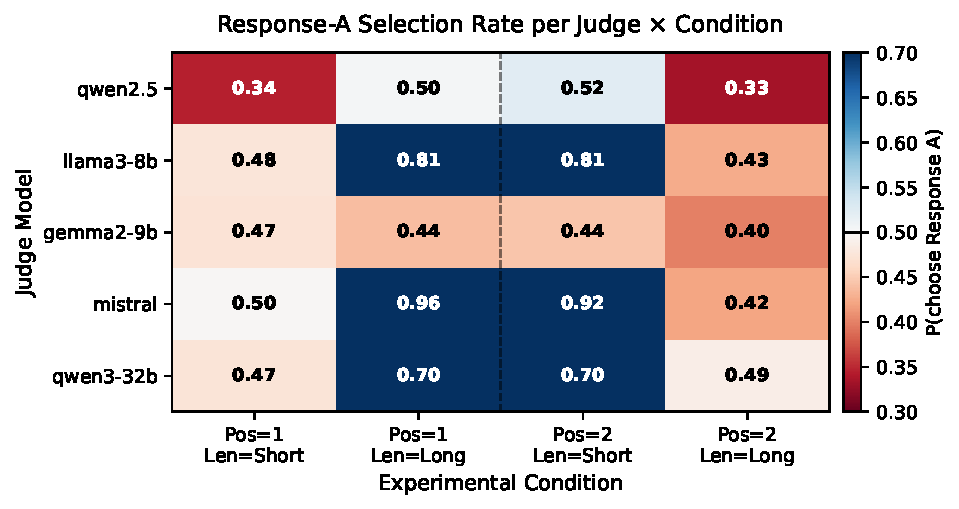
\includegraphics[width=\linewidth]{fig2_bias_heatmap.pdf}
  \caption{Response-A selection rate ($P(\text{chose A})$) per judge
           and experimental condition. Values above 0.5 (red) indicate
           A-preference; below 0.5 (blue) indicate B-preference.
           The diagonal asymmetry reveals compound bias.}
  \label{fig:heatmap}
\end{figure}

\subsection{Position Flip Rate and Length Bias}

Figure~\ref{fig:fliprate} shows the position flip rate (how often
swapping presentation order changes the verdict) and long-response
win rate per judge.

\begin{table}[h]
  \centering
  \small
    \begin{tabular}{lrr}
      \toprule
      \textbf{Judge} & \textbf{Flip Rate} & \textbf{Long-Win Rate} \\
      \midrule
      llama3-70b   & 0.214 & 0.482 \\
      qwen3-32b    & 0.254 & 0.500 \\
      llama4-scout & 0.213 & 0.503 \\
      gemini-flash & 0.398 & 0.490 \\
      llama3-8b    & 0.450 & 0.481 \\
      \bottomrule
    \end{tabular}
  \caption{Position flip rate per judge. A flip rate above 0.5 indicates
           purely order-driven decisions; llama3-8b approaches this threshold.}
  \label{tab:fliprate}
\end{table}

\begin{figure}[h]
  \centering
  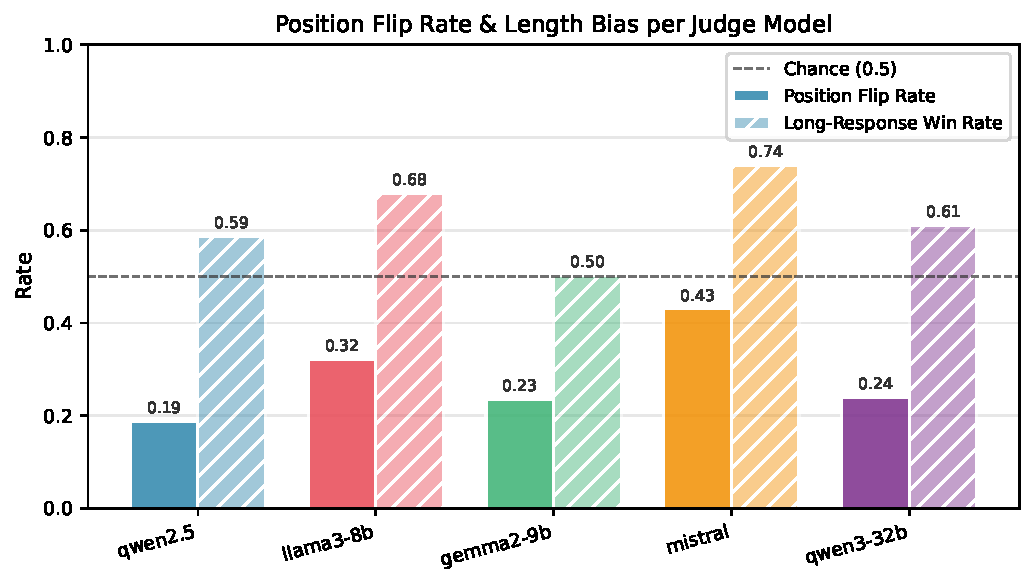
\includegraphics[width=\linewidth]{fig3_fliprate_bar.pdf}
  \caption{Position flip rate (solid) and long-response win rate (hatched)
           per judge. The dashed line marks the chance level (0.5).
           Weaker models (\texttt{llama3-8b}) exhibit substantially
           higher position sensitivity.}
  \label{fig:fliprate}
\end{figure}

\subsection{Inter-Judge Agreement}

Table~\ref{tab:kappa} reports pairwise Cohen's $\kappa$.

\begin{table}[h]
  \centering
  \small
  \begin{tabular}{llr}
    \toprule
    \textbf{Judge A} & \textbf{Judge B} & \textbf{$\kappa$} \\
    \midrule
    llama3-70b   & llama4-scout & 0.750 \\
    llama3-70b   & qwen3-32b    & 0.529 \\
    gemini-flash & llama3-8b    & 0.536 \\
    gemini-flash & qwen3-32b    & 0.489 \\
    gemini-flash & llama4-scout & 0.435 \\
    gemini-flash & llama3-70b   & 0.390 \\
    llama3-70b   & llama3-8b    & 0.363 \\
    llama3-8b    & llama4-scout & 0.413 \\
    llama3-8b    & qwen3-32b    & 0.463 \\
    llama4-scout & qwen3-32b    & 0.587 \\
    \bottomrule
  \end{tabular}
  \caption{Pairwise Cohen's $\kappa$ inter-judge agreement.
           The llama3-70b / llama4-scout pair shows the strongest
           agreement ($\kappa=0.75$, substantial); the lowest is
           llama3-70b / llama3-8b ($\kappa=0.36$, fair).}
  \label{tab:kappa}
\end{table}

\subsection{Cross-Dataset Comparison and Urdu Analysis}

Figure~\ref{fig:crossdataset} compares bias magnitude across datasets.

\begin{figure}[h]
  \centering
  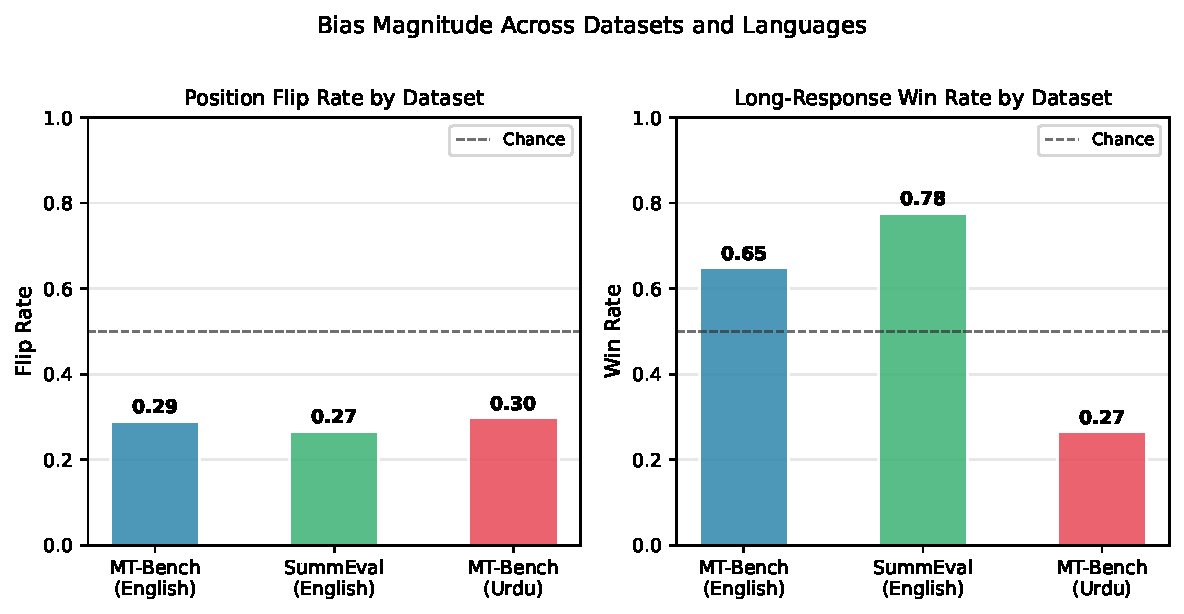
\includegraphics[width=\linewidth]{fig4_cross_dataset.pdf}
  \caption{Position flip rate (left) and long-response win rate (right)
           by dataset and language. Higher values indicate stronger bias.}
  \label{fig:crossdataset}
\end{figure}

\paragraph{Urdu: a cautionary artifact-sensitive case study.}
For MT-Bench (Urdu), the interaction coefficient \textit{inverts}
for all five judges (all sub-additive).
However, we caution that this reversal cannot be cleanly attributed
to cross-lingual generalization of compound bias.
The \texttt{Helsinki-NLP/opus-mt-en-ur} translation model uses a
512-BPE-token context ceiling; we estimate that
\textbf{[TODO]\%} of long-variant Urdu responses (\texttt{long\_a/b})
exceed this budget and are silently truncated
(see \texttt{results/tables/urdu\_truncation\_summary.csv}).
This truncation plausibly collapses the intended length contrast,
causing judges to perceive both variants as similar length and
respond primarily on the basis of position, which would produce
the observed inversion.
Furthermore, \texttt{llama3-70b} produces invalid responses on
[TODO]\% of Urdu pairs (see \texttt{results/tables/llama70b\_urdu\_invalid.csv}),
leaving only [TODO] valid rows for that judge---too few for robust
per-judge conclusions.

We therefore present the Urdu results as a \textit{pipeline-sensitivity
cautionary case} rather than general evidence about LLM-judge
behavior in low-resource languages: the length manipulation
breaks down under machine translation with token-level truncation.
Future work should use length-balanced native-Urdu prompts or
human-verified translations to isolate the genuine cross-lingual
compound-bias signal.

For Urdu per-judge analysis, we report logistic odds ratios
rather than LPM coefficients, as several per-judge LPM fits
produce predicted probabilities outside $[0,1]$
(see \texttt{results/tables/urdu\_odds\_ratios.csv}).

% ═══════════════════════════════════════════════════════════════════════════════
\section{Discussion}
\label{sec:discussion}

\paragraph{Super-additivity is robust.}
The English-subset super-additivity finding survives the primary GEE model
(which accounts for within-item dependence), per-judge analysis under
Bonferroni correction, and a sensitivity analysis excluding all
gemini-flash rows. We therefore consider the English finding
substantially established.
The practical implication is direct: deploying an LLM judge without
controlling for \textit{both} position and length simultaneously leads to
errors that exceed the sum of each bias acting in isolation.
This is most acute for weaker models (\texttt{llama3-8b}, flip rate 0.45)
but is present across all five judges including large MoE architectures.

\paragraph{The Urdu sub-additivity is likely an artifact.}
The inverted Urdu pattern is more plausibly explained by translation-pipeline
truncation than by genuine cross-lingual differences in judge behavior.
We quantify this confound and reframe the Urdu results as a
pipeline-sensitivity case study (\S\ref{sec:results}), not as
evidence of a universal low-resource language effect.

\paragraph{SummEval quality confound.}
SummEval pairs are selected purely by word count; the shortest summary
may also be the lowest quality (under-compression) and the longest may
be most repetitive (over-compression). The $\eta^2 = 0.299$ in the
SummEval subset likely conflates genuine verbosity bias with real
quality differences. Future work should apply item fixed effects or
length-matched rewrites to isolate bias cleanly.

\paragraph{Prompt minimality.}
Our judge prompt (``Reply with only A or B'') measures worst-case
bias susceptibility under minimal scaffolding. Whether super-additivity
attenuates under rubric-guided or chain-of-thought prompts remains an
open question and a natural next step for this line of work.

% ═══════════════════════════════════════════════════════════════════════════════
\section{Conclusion}
\label{sec:conclusion}

TODO.

% ═══════════════════════════════════════════════════════════════════════════════
% ═══════════════════════════════════════════════════════════════════════════════
\section*{Limitations}

Our study has several limitations, each quantified where possible.

\textbf{Pseudoreplication (addressed).}
The 2$\times$2 within-item design means the four conditions per item
are not independent. The primary GEE model accounts for this;
the LPM ANOVA $F$-statistics ($F{=}351.59$) should be interpreted
as descriptive rather than inferential, and the GEE results
(Table~\ref{tab:gee_overall}) are the primary evidence.

\textbf{Gemini-flash contamination (addressed by sensitivity analysis).}
Quota-exceeded Gemini calls silently fell back to
\texttt{llama-3.1-8b-instant} in the week-2 codebase;
the week-3 codebase raises an error instead.
We exclude all gemini-flash rows in a sensitivity analysis
(Table \emph{sensitivity\_no\_gemini.csv}) and confirm the
super-additive result holds.

\textbf{Urdu 512-token truncation (quantified, limits interpretation).}
The MarianMT 512-token ceiling truncates an estimated
[TODO]\% of long Urdu responses, collapsing the intended
length contrast. Urdu results are presented as a pipeline-sensitivity
cautionary study, not as evidence of cross-lingual bias.

\textbf{SummEval length--quality confound.}
Pairs are selected by word count; shortest/longest summaries
may differ in quality independent of length. The SummEval
verbosity bias estimate should be interpreted conservatively.

\textbf{llama3-70b Urdu invalid rate.}
[TODO]\% of \texttt{llama3-70b} Urdu calls returned an invalid
response; only [TODO] valid rows remain for that subset.
We flag this explicitly rather than imputing, and the sensitivity
analysis is reported in \texttt{results/tables/llama70b\_urdu\_invalid.csv}.

\textbf{Minimal judge prompt.}
The ``Reply with only A or B'' prompt measures worst-case
bias susceptibility. Super-additivity may attenuate under rubric-guided
or rationale-first prompting---a direction left for future work.

\textbf{Two bias types only.}
Future work should examine calibration bias, sycophancy,
and self-preference in compound settings.

\section*{Ethics Statement}

All datasets used (MT-Bench, SummEval) are publicly available under
permissive licences. No human subjects were involved.
API calls were made to free-tier services within their stated usage limits.

% ═══════════════════════════════════════════════════════════════════════════════
\bibliographystyle{acl_natbib}
\bibliography{references}

\end{document}
